\chapter{Elements of Point-Set Topology}
\label{ch:topology}

Point-set topology studies the properties of certain classes of sets that are
invariant under continuous transformations. Point-set topology gradually took
shape during the period from the late nineteenth century to the early
twentieth century.

If one wishes to study the properties of sets under continuous
transformations, the first problem to be solved is how to define a
``continuous'' map on a general set.

\section{Topological Spaces and Continuous Maps}
The prototype of a topological space is Euclidean space $\mathbb{R}^n$.
Besides being a set of points, Euclidean space carries many additional
structures, such as a metric, coordinates, an inner product, and an
orientation, all of which are irrelevant to topology. The idea behind the
notion of a topological space is to discard all properties unrelated to
continuous maps, thereby extracting the essence of continuity.

The concept of a continuous map was originally based on the notion of
distance: if $f:\mathbb{R}^n\to\mathbb{R}^m$ is a continuous map, then for
any $\mathbf{x}\in\mathbb{R}^n$ and any $\epsilon>0$, there exists a
$\delta >0$ such that for all $\mathbf{y}\in\mathbb{R}^n$ with
$||\mathbf{y}-\mathbf{x}||<\delta$, one has
$||f(\mathbf{y})-f(\mathbf{x})||<\epsilon$. However, the notion of distance
depends too heavily on Euclidean space, coordinates, and the like.

In fact, in courses on mathematical analysis or real variables, we may have
learned another characterization of continuous maps: $f$ is a continuous map
from $\mathbb{R}^n$ to $\mathbb{R}^m$ if and only if for every open set
$V\subset\mathbb{R}^m$, its preimage $f^{-1}(V)$ under $f$ is an open set in
$\mathbb{R}^n$. This equivalent characterization highlights the importance of
the notion of open sets for the notion of continuous maps.

But to define open sets, we still need the notion of distance in
$\mathbb{R}^n$. Indeed, the definition of an open set requires that every
point of the set have a ball centered at that point, with some positive radius
$r>0$, contained in the set. Therefore, without a thorough reformulation of
the notion of open sets, we still cannot bypass the notion of distance.

In fact, the notion of open sets leads to some basic properties of open sets.
For example, an arbitrary union of open sets is still open, and a finite
intersection of open sets is still open. So if we wish to define open sets
successfully while bypassing the notion of distance, a natural idea is to use
these basic properties of open sets as the means of characterizing them. From
this idea there arises naturally the approach of defining open sets on a
general set of points, namely the concept of a \underline{topological
structure} on a general set.


\begin{definition}[Topological Structure]
	Let $S$ be a nonempty set. A topology (structure) $\mathcal{T}$ on $S$ is
	a collection of subsets of $S$ such that the empty set $\emptyset$ and the
	set $S$ itself are in $\mathcal{T}$, and $\mathcal{T}$ is closed under
	\underline{arbitrary unions} and \underline{finite intersections}; that
	is, if $U_\alpha \in \mathcal{T}$ for all $\alpha\in I$ ($I$ being some
	index set), then $\bigcup_{\alpha\in I} U_\alpha \in \mathcal{T}$, and if
	$U_1,U_2,\cdots, U_n\in\mathcal{T}$, then
	$\bigcap_{i=1}^n U_i\in\mathcal{T}$.

	The elements of $\mathcal{T}$ are called \emph{open sets}, and the
	ordered pair $(S,\mathcal{T})$ is called a \emph{topological space}.

\end{definition}

\begin{remark}
	Sometimes we also simply call $S$ a topological space. A neighborhood of
	a point $p\in S$ is any open set $U\in \mathcal{T}$ containing $p$. If
	$\mathcal{T}_1$ and $\mathcal{T}_2$ are both topologies on the set $S$
	and $\mathcal{T}_1\subset \mathcal{T}_2$, then we say that
	$\mathcal{T}_1$ is coarser than $\mathcal{T}_2$; conversely, we say that
	$\mathcal{T}_2$ is finer than $\mathcal{T}_1$.
\end{remark}

\begin{example}[Different Topologies on a Finite Set]
	Let $S = \{a,b,c\}$.

	\begin{itemize}
		\item Let $\mathcal{T}_1 = \left\{\emptyset, S, \{a\},
			      \{b,c\}\right\}$. Then $(S,\mathcal{T}_1)$ is a topological space,
		      and $\{a\}$, $\{b,c\}$ are both open sets.
		\item Let $\mathcal{T}_0 = \left\{\emptyset, S\right\}$. Then
		      $(S,\mathcal{T}_0)$ is also a topological space, called the
		      \emph{trivial topological space} on $S$.
		\item Let $\mathcal{T}_2 = 2^S$. Then $(S,\mathcal{T}_2)$ is also a
		      topological space, called the discrete topological space on $S$.
		      Under this topology, every subset is an open set in $S$. Such a
		      topological space is called a \emph{discrete topological space}.
	\end{itemize}
	Clearly, from $\mathcal{T}_0$ to $\mathcal{T}_1$ to $\mathcal{T}_2$, the
	three topologies are increasingly fine.

\end{example}



\begin{example}[The Topology on Euclidean Space]
	The familiar definition of open sets in Euclidean space $\mathbb{R}^n$
	gives the \emph{standard topology} on Euclidean space. Under this
	topology, a set $U$ is called an open set in $\mathbb{R}^n$ if and only
	if for every $p\in U$, there exists an open ball $B(p,\epsilon)$
	centered at $p$ with radius $\epsilon$ contained in $U$. In what
	follows, unless otherwise stated, we will always use this standard
	topology.
\end{example}

\begin{remark} The description of open sets in $\mathbb{R}^n$ can be
	generalized to arbitrary topological spaces. See the exercises in
	\ref{exsec:top}, Proposition \ref{ex:open_criterion}.
\end{remark}

\begin{definition}[Closed Set]
	The complement of an open set is called a closed set.
\end{definition}

\begin{remark}
	By de Morgan's laws, an arbitrary intersection or a finite union of
	closed sets is still closed (see the exercises in \ref{exsec:top}).
	Because of the complementary relation between open and closed sets, we
	can also define a topological space using closed sets.
\end{remark}


\begin{example}[The Finite Complement Topology on $\mathbb{R}^1$]
	Let $\mathcal{T}$ be the collection of subsets of $\mathbb{R}^1$
	consisting of the empty set $\emptyset$, $\mathbb{R}^1$ itself, and the
	complements of finite sets. Let $F_\alpha$ and $F_i$ be finite sets,
	where $\alpha$ belongs to some index set $A$ and $i=1,2,\cdots,n$. Then
	by de Morgan's laws,
	\begin{displaymath}
		\bigcup_{\alpha} \left(\mathbb{R}^1-F_\alpha\right) = \mathbb{R}^1
		\smallsetminus \bigcap_{\alpha\in A} F_\alpha,\quad \text{and}
		\quad \bigcap_{i=1}^n \left(\mathbb{R}^1 - F_i\right) =
		\mathbb{R}^1 \smallsetminus \bigcup_{i=1}^n F_i.
	\end{displaymath}
	Since $\bigcap_{\alpha} F_\alpha$ and $\bigcup_{i=1}^n F_i$ are both
	finite sets, $\mathcal{T}$ is closed under arbitrary unions and finite
	intersections. Therefore $\mathcal{T}$ defines a topological space,
	called the \emph{finite complement topology}.
\end{example}


In fact, using the same idea, we can define the finite complement topology on
any set.

\begin{example}[The Zariski Topology]
	In algebraic geometry, the topology we often use is called the Zariski
	topology. Let $\mathbb{C}$ be the set of complex numbers. Let
	$S = \mathbb{C}^n$ be the complex $n$-dimensional vector space. A subset
	of $\mathbb{C}^n$ is called a (Zariski) closed set if it is the solution
	set of finitely many polynomial equations $P_1,P_2,\cdots, P_r$ in $n$
	variables with complex coefficients. We leave the verification of the
	closed-set properties of this topology as an exercise.
\end{example}

We will now generalize the notion of continuous maps to topological spaces,
modeled on the definition of continuous maps on Euclidean space. Note that
this generalization of continuity does not depend on the notion of a metric,
but is based entirely on open sets.

Recall the notion of a continuous map: let $f:\mathbb{R}^n\to\mathbb{R}^m$ be
a continuous map; then for every point $p\in\mathbb{R}^n$ and every
neighborhood $V$ of $f(p)$ (for example $B(f(p),\epsilon)$), there exists a
neighborhood $U$ of $p$ (for example $B(p,\delta)$) such that
$f(U)\subset V$. This property leads to the following proposition.




\begin{proposition}[Continuity in the Language of Open Sets]
  Let $f:X\to Y$ be a map between topological spaces $X$ and $Y$. Then $f$
	is a continuous map if and only if the preimage $f^{-1}(V)$ of every open
	set $V$ in $Y$ under $f$ is an open set in $X$.
\end{proposition}

\begin{proof} \quad

	\begin{itemize}
		\item [$\Longrightarrow$] Let $V$ be an arbitrary open set in $Y$. To
		      show that $f^{-1}(V)$ is an open set in $X$, we take an arbitrary
		      point $p$ in $f^{-1}(V)$. Then $f(p)\in V$. Since $f$ is known to
		      be continuous, there exists an open set $U$ in $X$ containing $p$
		      such that $f(U)\subset V$. Hence $p\in U\subset f^{-1}(V)$. By the
		      local criterion for openness (Exercise \ref{ex:open_criterion}),
		      $f^{-1}(V)$ is an open set in $X$.

		\item [$\Longleftarrow$] Let $p$ be a point in the topological space
		      $X$. We need to show that for every neighborhood $V$ of $f(p)$,
		      there exists a neighborhood $U$ of $p$ such that $f(U)\subset V$.
		      By hypothesis, $f^{-1}(V)$ itself satisfies the requirement.
		      Therefore $f$ is a continuous map.
	\end{itemize}

\end{proof}




Remark: the above proposition in fact gives the definition of a continuous map
between topological spaces.




\begin{definition}[Continuous Maps Between Topological Spaces]
	A map $f:X\to Y$ between topological spaces $X$ and $Y$ is continuous if
	and only if the preimage under $f$ of every open set is open.
\end{definition}


\begin{example}[Continuity of the Inclusion Map]
	Let $A$ be a subspace of $X$ (the notion of a subspace is introduced in
	Section \ref{subsec:subspace_top}). Then the inclusion map $i:A\to X$,
	$i(a)=a$, is continuous.
\end{example}


\begin{example}[Continuity of Projection Maps] Let $\pi: X\times Y\to X$,
	$\pi(x,y) = x$ be the projection. Then $\pi$ is a continuous map. (The
	notion of a product topological space is introduced in Section
	\ref{subsec:product_top}.)

\end{example}

\begin{proposition}[Composition of Continuous Maps]
	If $f:X\to Y$ and $g:Y\to Z$ are continuous maps, then $g\circ f: X\to
		Z$ is continuous.
\end{proposition}

The proof is left as an exercise.


Let $A$ be a subspace of $X$ and $f:X\to Y$ a map. We define the restriction
of $f$ to the set $A$, denoted $f|_A:A\to Y$, by $(f|_A)(a) = f(a)$. In fact,
if $i:A\to X$ denotes the inclusion map, then the restriction map can be
written as $f\circ i$.


\begin{corollary}
	The restriction $f|_A$ of a continuous map $f:X\to Y$ to a subspace
	$A\subset X$ is also continuous.
\end{corollary}


\begin{proposition}[Continuity Defined via Closed Sets]
	A map $f:X\to Y$ is continuous if and only if the preimage of every
	closed set is closed.

\end{proposition}

The proof is left as an exercise.


\begin{definition}[Open Maps and Closed Maps]
	A map $f:X\to Y$ is called an open map if the image of every open set in
	$X$ is an open set in $Y$; similarly, $f:X\to Y$ is called a closed map
	if the image of every closed set in $X$ is a closed set in $Y$.
\end{definition}


\begin{definition}[Homeomorphism] A continuous bijection $f$ from $X$ to $Y$
	whose inverse map is also continuous is called a homeomorphism
	$f:X\to Y$. The topological spaces $X$ and $Y$ are then said to be
	homeomorphic.

\end{definition}



\subsection{Exercises} \label{exsec:top}

\begin{enumerate}
	\item
    \begin{proposition}[Local Criterion for Openness]
      \label{ex:open_criterion} Let $S$ be a topological space. Prove that
		      a subset $A$ is open in $S$ if and only if for every $p\in A$, there
		      exists an open set $V$ such that $p\in V\subset A$.
	    \end{proposition}

	\item
	      Prove that in a topological space $S$, an arbitrary intersection of
	      closed sets is closed, and a finite union of closed sets is closed.

	\item Let $Z_\alpha$, $Z_i$ be solution sets of finite families of
	      polynomials in $\mathbb{C}^n$. Prove that $\bigcup_\alpha Z_\alpha$
	      and $\bigcap_{i=1}^m Z_i$ are again solution sets of finite families
	      of polynomials.


	\item  If $f:X\to Y$ and $g:Y\to Z$ are continuous, then $g\circ f: X\to
		      Z$ is continuous.


	\item A map $f:X\to Y$ is continuous if and only if the preimage of every
	      closed set is closed.

\end{enumerate}


%%%%%%%%%%%%%%%%%%%%%%%%%%%%%%%%%%%%%%%%%%%%%%%%%%%%%%%%%%%%%%%%%%%%%%%%%%%%%%%%




\newpage

\section{Subspace Topology}\label{subsec:subspace_top}

Let $(S,\mathcal{T})$ be a topological space and $A$ a subset of $S$. Define
$\mathcal{T}_A$ to be the collection of subsets
\begin{displaymath}
	\mathcal{T}_A = \left\{U\cap A\; | \; U\in\mathcal{T}\right\}.
\end{displaymath}
By the distributive laws of set operations, one can show that $\mathcal{T}_A$
is closed under arbitrary unions and finite intersections, and that
$\emptyset,A \in\mathcal{T}_A$. Therefore $\mathcal{T}_A$ is a topology on
the set $A$, called the \emph{subspace topology}, or the relative topology of
$A$ in $S$, and the elements of $\mathcal{T}_A$ are called open sets in $A$.
Note that a set $U$ that is open in $A$ need not be open in $S$. In this
situation we also say that $U$ is relatively open in $A$, or open relative to
$A$. A subset $A$ of $S$ endowed with the subspace topology $\mathcal{T}_A$
is called a subspace of $S$.


\begin{example}
	Let $A = [0,1]\subset \mathbb{R}^1$. Then $A$ can be made into a
	subspace of $\mathbb{R}^1$: it suffices to declare the relatively open
	sets in $A$ to be the intersections of open sets of $\mathbb{R}^1$ with
	$A$. For example, $[0,\frac12)\subset A$ is an open set relative to $A$,
	since it can be written as $(-\frac12,\frac12)\cap A$. See Figure
	\ref{fig:relative_open}.
	\begin{figure}[!ht]
		\centering
		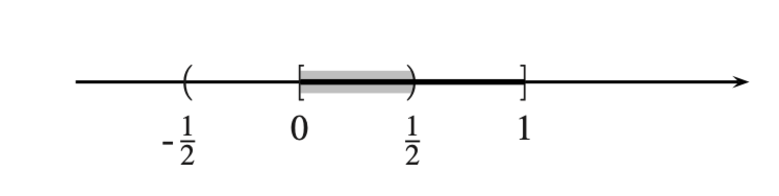
\includegraphics[width=0.5\textwidth]{figures/relative_open}
    \caption{A relatively open set (quoted from
			\cite{tu_introduction_2011})}
		\label{fig:relative_open}
	\end{figure}
\end{example}


%%%%%%%%%%%%%%%%%%%%%%%%%%%%%%%%%%%%%%%%%%%%%%%%%%%%%%%%%%%%%%%%%%%%%%%%%%%%%%%%

\newpage



\section{Bases}

In general, it is fairly difficult to describe all the open sets in a topology
$\mathcal{T}$ explicitly. Usually, however, we can describe a subcollection
$\mathcal{B}$ of $\mathcal{T}$ such that every open set in $\mathcal{T}$ can
be expressed as a union of open sets in $\mathcal{B}$.

\begin{definition}[Basis of a Topology] A subcollection $\mathcal{B}$ of a
	topology $\mathcal{T}$ is a basis for $\mathcal{T}$ if, given any open
	set $U$ and any point $p$ in $U$, there is always an open set
	$B\in\mathcal{B}$ in $\mathcal{B}$ such that $p\in B\subset U$. We also
	say that $\mathcal{B}$ generates the topology $\mathcal{T}$, or that
	$\mathcal{B}$ is a basis for the topological space $S$.

\end{definition}




\begin{example}
	The collection of all open balls $B(p,r)$ in $\mathbb{R}^n$ is a basis
	for the standard topology on $\mathbb{R}^n$, where $p\in\mathbb{R}^n$ is
	any point and $r$ is any positive real number.
\end{example}



\begin{proposition} A collection of open sets $\mathcal{B}$ is a basis for $S$
	if and only if every open set in $S$ can be written as a union of sets in
	$\mathcal{B}$. (The empty set is regarded as the union of zero sets from
	$\mathcal{B}$.)
\end{proposition}

\begin{proof}\quad

	\begin{itemize}
		\item [$\Longrightarrow$] Suppose $\mathcal{B}$ is a basis and $U$ is
		      an arbitrary open set in $S$. For each point $p\in U$, there exists
		      at least one open set $B_p\in \mathcal{B}$ such that $p\in B_p
			      \subset U$. Hence $U=\bigcup_{p\in U}B_p$.

		\item [$\Longleftarrow$] Suppose every open set in $S$ can be written
		      as a union of sets in $\mathcal{B}$. Given an open set $U$ and an
		      arbitrary point $p$ in $U$, since $U$ can be written as a union of
		      sets in $\mathcal{B}$, there must exist a $B_\alpha\in \mathcal{B}$
		      such that $p\in B_\alpha \subset U$. Therefore $\mathcal{B}$ is a
		      basis.
	\end{itemize}
\end{proof}

The following proposition gives a criterion for whether a collection
$\mathcal{B}$ can serve as a basis for some topology.

\begin{proposition}[Criterion for a Basis]
  \label{prop:criterion bases}
	A collection $\mathcal{B}$ of subsets of a set $S$ is a basis for some
	topology $\mathcal{T}$ on $S$ if and only if
	\begin{enumerate}
		\item $S$ is the union of all the sets in $\mathcal{B}$, and
		\item given any two sets $B_1, B_2\in\mathcal{B}$ and any point $p\in
			      B_1\cap B_2$, there exists a set $B\in \mathcal{B}$ such that $p\in
			      B\subset B_1\cap B_2$. See Figure \ref{fig:criterion_bases}.
	\end{enumerate}
\end{proposition}

\begin{figure}[h!]
	\centering
	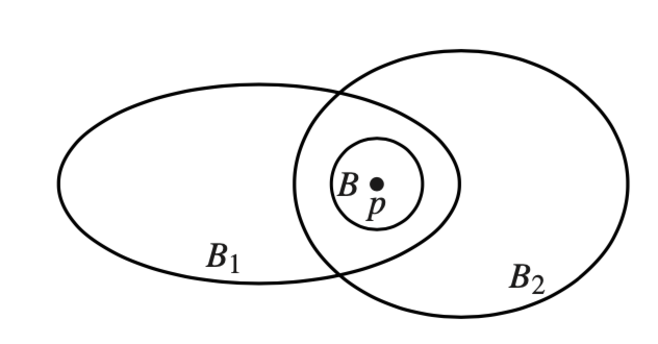
\includegraphics[width=0.5\textwidth]{figures/criterion_bases}
	\caption{The criterion for a basis, from \cite{tu_introduction_2011}}
	\label{fig:criterion_bases}
\end{figure}




\begin{proof}
	($\Longrightarrow$) If the collection $\mathcal{B}$ is a basis for some
	topology $\mathcal{T}$, then of course
	\begin{enumerate}
		\item the whole set $S$ is an open set, and hence can be written as a
		      union of sets in $\mathcal{B}$;
		\item since the sets in $\mathcal{B}$ are all open, for any $B_1, B_2
			      \in\mathcal{B}$ their intersection $B_1\cap B_2$ is also open; if
		      there exists $p\in B_1\cap B_2$, then by the definition of a basis,
		      there exists $B\in\mathcal{B}$ such that $p\in B\subset B_1\cap
			      B_2$.

		      ($\Longleftarrow$) Suppose there is a collection $\mathcal{B}$
		      satisfying conditions 1 and 2. We now construct a collection
		      $\mathcal{T}$ consisting of arbitrary unions of sets in
		      $\mathcal{B}$. We will verify below that $\mathcal{T}$ satisfies
		      all the properties required of a topology.

		      First, $\emptyset$ (the union of zero sets) and $S$ (by condition
		      1) are in $\mathcal{T}$. Second, $\mathcal{T}$ is obviously closed
		      under unions. Finally, it suffices to show that $\mathcal{T}$ is
		      closed under finite intersections. By mathematical induction, it
		      suffices to show that if $U,V\in\mathcal{T}$, then $U\cap
			      V\in\mathcal{T}$. Write $U$ and $V$ as unions of sets in
		      $\mathcal{B}$:
		      \begin{displaymath}
			      U = \bigcup_{\alpha}U_\alpha,\quad V = \bigcup_{\beta} V_\beta
		      \end{displaymath}
		      Then
		      \begin{displaymath}
			      U\cap V = \bigcup_{\alpha,\beta} (U_\alpha \cap V_\beta).
		      \end{displaymath}
		      For any $p\in U\cap V$, there exist some $\alpha$ and $\beta$ such
		      that $p\in U_\alpha\cap V_\beta$. By condition 2, there exists
		      $B_p\in\mathcal{B}$ such that $p\in B_p\subset U_\alpha\cap
			      V_\beta$. Hence
		      \begin{displaymath}
			      U\cap V = \bigcup_{p\in U\cap V} B_p \in\mathcal{T}.
		      \end{displaymath}

	\end{enumerate}
\end{proof}




\begin{proposition}
	Let $\mathcal{B} = \{B_\alpha\}$ be a basis for the topological space
	$S$, and let $A$ be a subspace of $S$. Then $\{B_\alpha\cap A\}$ is a
	basis for $A$.
\end{proposition}


The proof is left to the reader as an exercise.



\subsection{First and Second Countability}

First and second countability, as the names suggest, concern the countability
of bases.


\begin{lemma}
	Every open set in $\mathbb{R}^n$ contains a point all of whose
	coordinates are rational.
\end{lemma}


\begin{proposition}
	The collection $\mathcal{B}_{\text{rat}}$ of all open balls with
	rational centers and rational radii is a basis for $\mathbb{R}^n$.

\end{proposition}

\begin{definition}
	A topological space is said to be \emph{second countable} if it has a
	\underline{countable basis}.
\end{definition}

\begin{definition}
	Let $S$ be a topological space and $p$ a point of $S$. A
	\emph{neighborhood basis} at $p$ is a collection $\mathcal{B} =
		\{B_\alpha\}$ of neighborhoods of $p$ such that for every neighborhood
	$U$ of $p$, there exists a $B_\alpha\in\mathcal{B}$ with $p\in B_\alpha
		\subset U$. A topological space $S$ is said to be \emph{first
		countable} if it has a countable neighborhood basis at every point
	$p\in S$.
\end{definition}

\begin{example}
	For $p\in\mathbb{R}^n$, let $B(p,\frac1n)$ be the open ball centered at
	$p$ with radius $1/n$. Then $\{B(p,\frac1n)\}_{n=1}^\infty$ is a
	neighborhood basis at $p$. Hence $\mathbb{R}^n$ is a first countable
	topological space.
\end{example}


\begin{example}
	An uncountable discrete topological space is first countable but not
	second countable. Every second countable topological space is first
	countable (the proof is left as an exercise).
\end{example}

If $p$ is a point of a first countable topological space and
$\{V_i\}_{i=1}^\infty$ is a countable neighborhood basis at $p$, then setting
$U_i = V_1 \cap \cdots \cap V_i$, we obtain a countable descending sequence
\begin{displaymath}
	U_1 \supset U_2 \supset U_3 \supset \cdots
\end{displaymath}
which is still a neighborhood basis at $p$. Therefore, in giving the
definition of first countability, we may always assume that the countable
neighborhood basis at each point forms a descending sequence of open sets.




\subsection{Exercises} \label{exsec:bases}
\begin{enumerate}

	\item Prove: let $\mathcal{B} = \{B_\alpha\}$ be a basis for the
	      topological space $S$, and let $A$ be a subspace of $S$. Then
	      $\{B_\alpha\cap A\}$ is a basis for $A$.


	\item An uncountable discrete topological space is first countable but not
	      second countable. Every second countable topological space is first
	      countable.
\end{enumerate}

\newpage

\section{Separation Axioms}
There are many formulations of the separation axioms, but in these notes we
need only discuss the Hausdorff separation property and normality.

\begin{definition}[Hausdorff Topological Spaces]
	A topological space $S$ is called a \emph{Hausdorff} space if, given any
	two points $x,y\in S$, there always exist two disjoint open sets $U$ and
	$V$ such that $x\in U$ and $y\in V$. A Hausdorff space is called
	\emph{normal} if, given any two disjoint closed sets $F, G$, there exist
	disjoint open sets $U$, $V$ such that $F\subset U$ and $G\subset V$.

\end{definition}

\begin{figure}[h!]
	\centering
	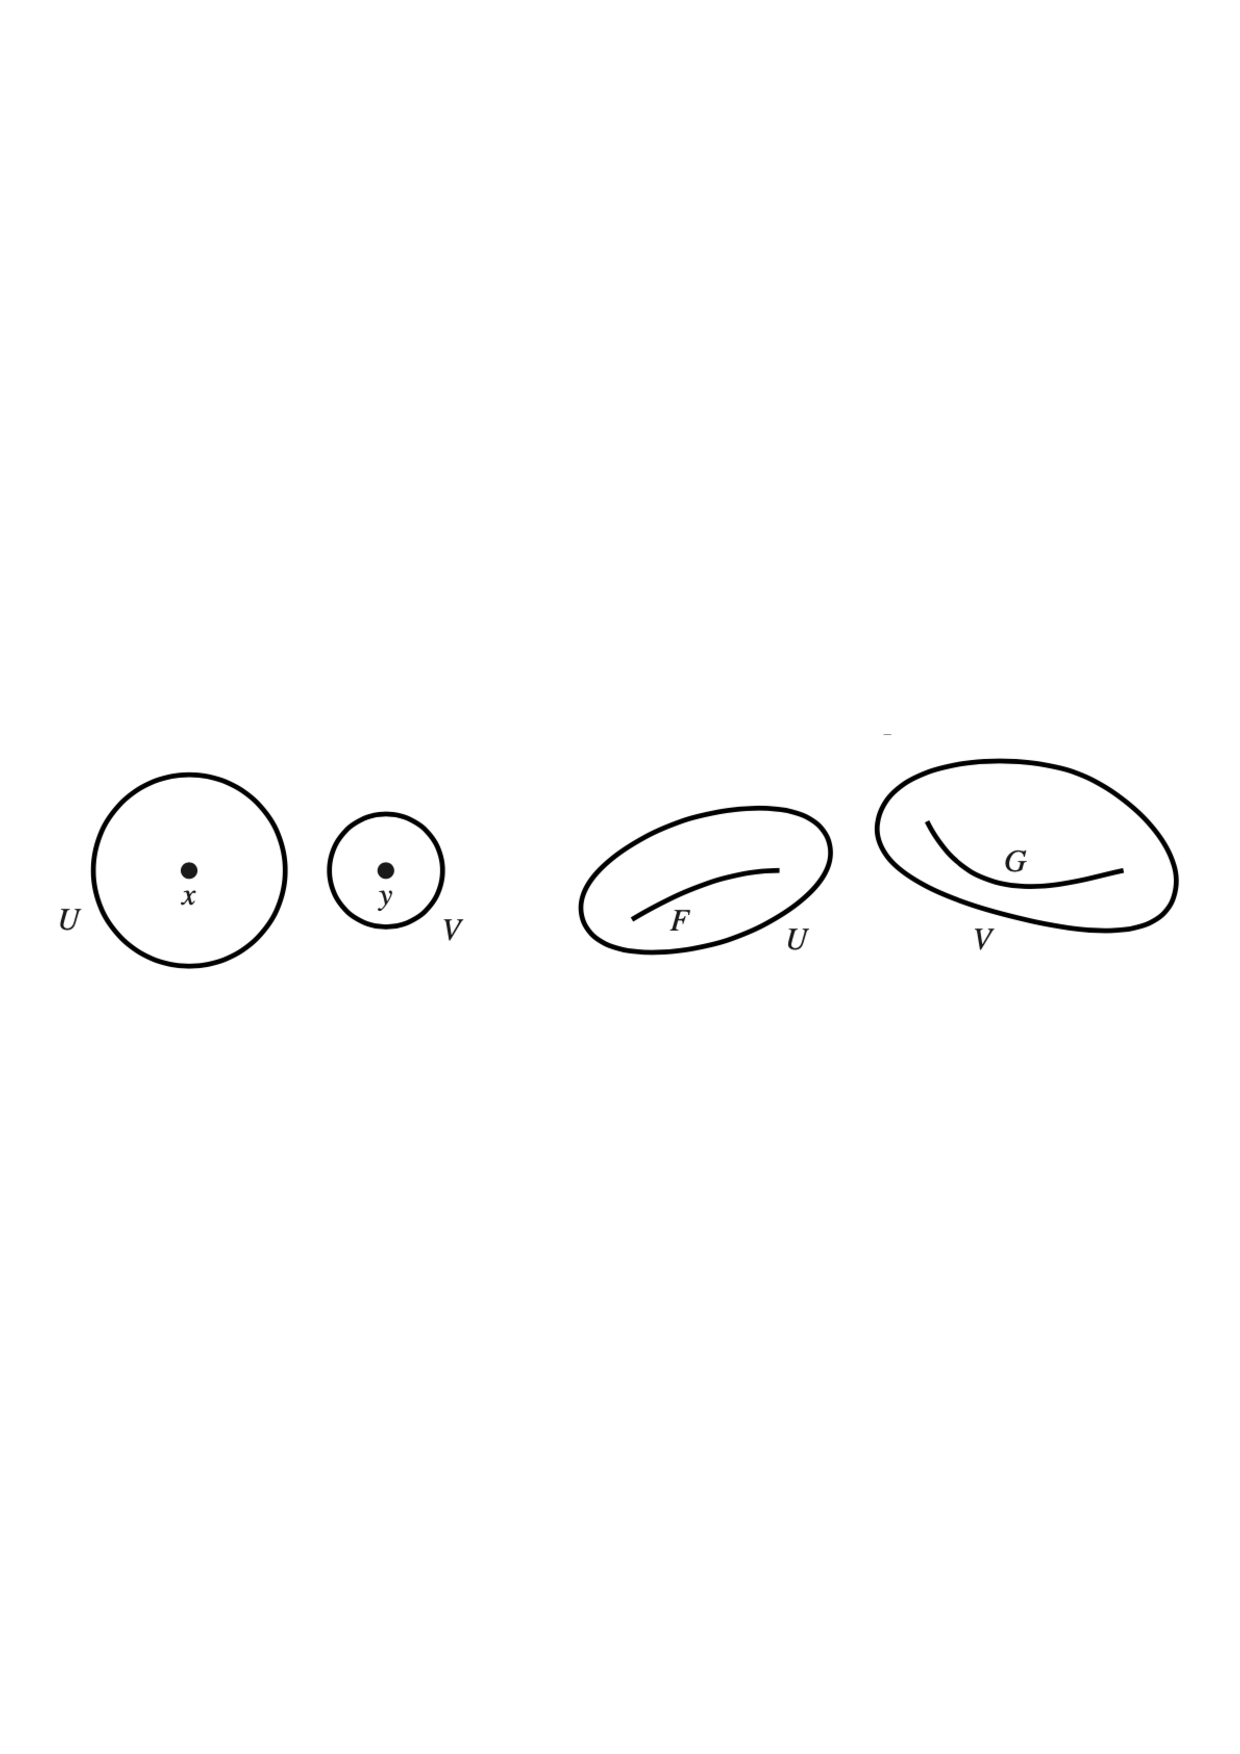
\includegraphics[width=0.5\textwidth]{figures/hausdorff_condition}
	\caption{The Hausdorff condition and normality, from
		\cite{tu_introduction_2011}}
	\label{fig:hausdorff_cond}
\end{figure}



\begin{proposition}
	Every one-point set in a Hausdorff space is closed.
\end{proposition}

The proof is left as an exercise.

\begin{example}[The Euclidean Topology]
	Euclidean space $\mathbb{R}^n$ is a Hausdorff space, because given any
	two distinct points $x,y\in\mathbb{R}^n$, if we take $\epsilon =
		\frac12 d(x,y)$, then the two open balls $B(x,\epsilon)$ and
	$B(y,\epsilon)$ will have no point in common.
\end{example}


\begin{example}[The Zariski Topology]
	Let $S = \mathbb{C}^n$ be the $n$-dimensional vector space over the
	field $\mathbb{C}$, endowed with the Zariski topology. Every open set
	$U$ is of the form $S\smallsetminus Z(I)$, where $I$ is a family of
	polynomials in $n$ variables and $Z(I)$ is the solution set of this
	family. In the Zariski topology, any two nonempty open sets intersect:
	if $U= S\smallsetminus Z(I)$ and $V = S\smallsetminus Z(J)$ are both
	nonempty, then
	\begin{displaymath}
		U\cap V = S\smallsetminus (Z(I)\cup Z(J))
	\end{displaymath}
	is nonempty (since $Z(I) \cup Z(J)$, being the solution set of $I$ or
	$J$, cannot be the whole space). Hence $\mathbb{C}^n$ with the Zariski
	topology is not Hausdorff.
\end{example}


\begin{proposition} Every subspace $A$ of a Hausdorff space $S$ is also
	Hausdorff.

\end{proposition}

The proof is left as an exercise.

\subsection{Exercises} \label{exsec:seperable}

\begin{enumerate}
	\item Prove that every one-point set in a Hausdorff space is closed.
	\item Prove that every subspace $A$ of a Hausdorff space $S$ is also
	      Hausdorff.
\end{enumerate}


\newpage


\section{Product Topology}\label{subsec:product_top}

Given two nonempty sets $A,B$, we can consider the Cartesian product set
$A\times B$, consisting of all ordered pairs $(a,b)$ with $a\in A$, $b\in B$.
Likewise, given two topological spaces $X$ and $Y$, we can consider the
product topological space $X\times Y$, again consisting of all ordered pairs
$(x,y)$ ($x\in X$, $y\in Y$). We only need to define a topology on $X\times
	Y$ that makes it a topological space. We construct the collection
$\mathcal{B}$ consisting of all sets of the form $U\times V$, where $U$ and
$V$ are open sets in $X$ and $Y$ respectively. We call the sets in
$\mathcal{B}$ basic open sets in $X\times Y$.

If $U_1\times V_1$ and $U_2\times V_2$ are both in $\mathcal{B}$, then
\begin{displaymath}
	(U_1\times V_1)\cap (U_2\times V_2) = (U_1\cap U_2)\times (V_1\cap
	V_2)
\end{displaymath}
is also in $\mathcal{B}$. From this we see that $\mathcal{B}$ generates a
topology, called the product topology. Unless otherwise stated, we will always
use this topology on product spaces.


\begin{proposition}
	Let $\{U_i\}$ and $\{V_j\}$ be bases for the topological spaces $X$ and
	$Y$ respectively. Then $\{U_i\times V_j\}$ is a basis for $X\times Y$.
\end{proposition}

The proof is left as an exercise.


\begin{corollary}
	The product of two second countable topological spaces is second
	countable.
\end{corollary}
Clearly; the proof is omitted.


\begin{proposition}
	The product of two Hausdorff topological spaces is Hausdorff.
\end{proposition}

The proof is left as an exercise.

\subsection{Exercises}

\begin{enumerate}
	\item   Let $\{U_i\}$ and $\{V_j\}$ be bases for the topological spaces
	      $X$ and $Y$ respectively. Then $\{U_i\times V_j\}$ is a basis for
	      $X\times Y$.


	\item  The product of two Hausdorff topological spaces is Hausdorff.
\end{enumerate}


\newpage


\section{Compactness}
As in mathematical analysis, we can discuss when a topological space is
compact. Let $S$ be a topological space. A collection of open sets
$\{U_\alpha\}$ in $S$ is called a \emph{cover} (or \emph{open cover}) of $S$
if $S = \bigcup_\alpha U_\alpha$. If a subcollection
$\{U_\alpha\}_{\alpha\in\mathcal{B}\subset\mathcal{A}}$ of
$\{U_\alpha\}_{\alpha\in \mathcal{A}}$ still covers $S$, the subcollection is
called a \emph{subcover} of $S$.

\begin{definition}[Compact Topological Spaces]
	A topological space $S$ is called compact if every open cover of $S$ has
	a finite subcover.
\end{definition}

Via the subspace topology, a subset $A$ of a topological space $S$ is also a
topological space. The subspace $A$ can be covered by open sets of $A$, and
also by open sets of $S$. An open cover of $A$ in $S$ means a collection of
open sets $\{U_\alpha\}$ of $S$ whose union contains $A$. In this sense, $A$
is a compact set in $S$ if and only if every open cover of $A$ in $S$ has a
finite subcover.

\begin{proposition}
	A closed subset of a compact topological space is compact.
\end{proposition}

\begin{proposition}
	A compact subset $K$ of a Hausdorff topological space $S$ and a point
	$p$ outside the set can be separated by open sets; that is, there exist
	an open set $U\supset K$ and an open set $V\ni p$ such that $U\cap
		V=\emptyset$.
\end{proposition}


\begin{proposition}
	Every compact subset $K$ of a Hausdorff space $S$ is closed.
\end{proposition}


\begin{proposition}
	The image of a compact set under a continuous map is compact.
\end{proposition}


\begin{proposition}
	A continuous map from a compact topological space $X$ to a Hausdorff
	space $Y$ is a closed map.
\end{proposition}



\begin{corollary}\label{cor:from-compact-to-hausdorff}
	A continuous bijection $f$ from a compact topological space $X$ to a
	Hausdorff space $Y$ is a homeomorphism.
\end{corollary}



\begin{theorem}[Tychonoff] The product of an arbitrary family of compact
	spaces, endowed with the product topology, is compact.
\end{theorem}

% \section{Boundedness}

\newpage

\section{Connectedness}
\begin{definition}[Connected Topological Spaces]
	A topological space $S$ is called connected if there do not exist two
	nonempty disjoint open subsets $U$ and $V$ such that $S = U\cup V$. A
	subset $A$ of $S$ is called connected if it is connected as a
	topological subspace.
\end{definition}

\begin{proposition}
	A subset $A$ of a topological space $S$ is disconnected if and only if
	there exist open subsets $U$ and $V$ of $S$ such that
	\begin{itemize}
		\item $U\cap A\neq \emptyset$, $V\cap A \neq \emptyset$,
		\item $U\cap V \cap A = \emptyset$,
		\item $A\subset U\cup V$.
	\end{itemize}
	A pair of open sets with the above properties is called a separation of
	$A$.
\end{proposition}

\begin{figure}[h]
	\centering
	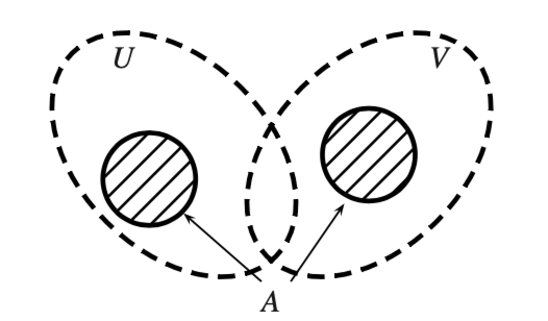
\includegraphics[width=0.5\textwidth]{figures/separation.pdf}
	\caption{A separation of $A$}
\end{figure}

\begin{proposition}
	The image of a connected topological space $X$ under a continuous map
	$f:X\to Y$ is connected.
\end{proposition}

\begin{proof}

\end{proof}

\begin{proposition}
	In a topological space $S$, the union of a family of connected subsets
	$A_\alpha$ having a common point $p$ is connected.
\end{proposition}

\subsection{Connected Components}
Let $x$ be a point of a topological space $S$. The set $C_x$ is the union of
all connected subsets of $S$ containing $x$; it is called the \emph{connected
	component} of $S$ containing $x$.


  \begin{proposition}
	Let $C_x$ be the connected component of a topological space $S$
	containing $x$. Then a connected subset $A\subset S$ is either disjoint
	from $C_x$ or entirely contained in $C_x$.
\end{proposition}

Thus a connected component is a maximal connected subset containing $x$.


\begin{corollary}
	For any two points $x$ and $y$ in a topological space $S$, their
	connected components $C_x$ and $C_y$ are either identical or disjoint.
\end{corollary}

As a consequence of the above corollary, the connected components of $S$
partition $S$ into disjoint subsets.


\newpage

\section{Closure}
Let $S$ be a topological space and $A$ a subset of $S$.

\begin{definition}[Closure]
	The \emph{closure} of $A$ in $S$, denoted $\overline{A}$, or $\cl(A)$,
	or $\cl_S(A)$, is defined as the intersection of all closed sets
	containing $A$.
\end{definition}

It follows from the definition that the closure is necessarily a closed set.
It is the smallest closed set containing $A$ (since every closed set
containing $A$ contains the closure).


\begin{proposition}[Local Characterization of the
	Closure]\label{prop:closure_local}
	Let $A$ be a subset of a topological space $S$. A point $p\in S$ lies in
	the closure $\cl(A)$ if and only if every neighborhood of $p$ contains
	at least one point of $A$.
\end{proposition}

\begin{proof} We will consider the contrapositive of the statement:
	\begin{displaymath}
		p\not\in \cl(A) \Longleftrightarrow \text{there exists a neighborhood
			of $p$ disjoint from $A$}
	\end{displaymath}

	($\Longrightarrow$) Suppose
	\begin{displaymath}
		p\not\in \cl(A) = \bigcap \{F | \text{$F$ is closed in $S$ and
			$F\supset A$}\}.
	\end{displaymath}
	Then $p$ fails to lie in some closed set containing $A$; that is, $p\in
		S\smallsetminus F$, an open set disjoint from $A$.

	($\Longleftarrow$) Suppose $p$ lies in an open set $U$ disjoint from
	$A$. Then the complement $F:=S\smallsetminus U$ is a closed set
	containing $A$ but not $p$. Hence $p\not\in \cl(A)$.

\end{proof}

\begin{example} The closure of the open disk $B(\mathbf{0},r)$ in
	$\mathbb{R}^2$ is the closed disk $\overline{B}(\mathbf{0},r) =
		\{p\in\mathbb{R}^2 \,|\, d(p,\mathbf{0})\le r \}$.

\end{example}

\begin{definition}
	A point $p$ in $S$ is called an \emph{accumulation point} of $A$ if
	every neighborhood of $p$ in $S$ contains a point of $A$ other than $p$.
	The set of all accumulation points of $A$ is denoted $\ac(A)$.
\end{definition}


Let $U$ be a neighborhood of $p$ in $S$; we call $U\smallsetminus\{p\}$ a
\emph{punctured neighborhood} of $p$. Then an equivalent condition for $p$ to
be an accumulation point of $A$ is that every punctured neighborhood of $p$
contains a point of $A$. In some books, an accumulation point is also called a
limit point.

\begin{example}
	If $A=[0,1)\cup\{2\}\subset\mathbb{R}^1$, then the closure of $A$ is
	$[0,1]\cup\{2\}$, but the set of accumulation points of $A$ is the
	closed interval $[0,1]$.
\end{example}

\begin{proposition}
	Let $A$ be a subset of a topological space $S$. Then
	\begin{displaymath}
		\cl(A) = A \cup \ac(A).
	\end{displaymath}
\end{proposition}

\begin{proof}

	($\supset$) By definition, $A\subset \cl(A)$. By the local
	characterization of the closure, $\ac(A)\subset\cl(A)$. Hence $A\cup
		\ac(A) \subset \cl(A)$.

	($\subset$) Let $p\in\cl(A)$. Then either $p\in A$ or $p\not\in A$. If
	$p\in A$, then $p\in A\cup \ac(A)$. Suppose $p\not\in A$. By Proposition
	\ref{prop:closure_local}, every neighborhood of $p$ contains a point of
	$A$ different from $p$ (since $p\not\in A$). Hence every punctured
	neighborhood of $p$ contains a point of $A$. Therefore
	\begin{displaymath}
		p\in \ac(A) \subset A\cup \ac(A).
	\end{displaymath}
	Thus $\cl(A)\subset A\cup \ac(A)$.

\end{proof}

\begin{proposition}
	A set $A$ is closed if and only if $A=\overline{A}$.
\end{proposition}


\begin{proposition}
	If $A\subset B$, then $\overline{A}\subset\overline{B}$.
\end{proposition}


\subsection{Exercises}
\begin{enumerate}
	\item Closures of finite unions and intersections. Let $A$ and $B$ be
	      subsets of a topological space $S$. Prove:
	      \begin{enumerate}
		      \item [(a)] $\overline{A\cup B} = \overline{A} \cup \overline{B}$,
		      \item [(b)] $\overline{A\cap B} \subset \overline{A}\cap
			            \overline{B}$.
	      \end{enumerate}
	      Consider $A=(a,0)$, $B=(0,b)\subset\mathbb{R}$; then in general
	      $\overline{A\cap B} \neq \overline{A} \cap \overline{B}$.

\end{enumerate}


\newpage

\section{Convergence}

Let $S$ be a topological space. A \emph{sequence} in $S$ is a map from
$\mathbb{Z}^+$ to $S$. We denote a sequence by $\{x_i\}$, or by
$x_1,x_2,x_3,\cdots$.

\begin{definition}
	A sequence $\{x_i\}$ converges to a point $p$ if for every neighborhood
	$U$ of $p$, there exists a positive integer $N$ such that $x_i\in U$ for
	all $i\ge N$. In this case we say that $p$ is a limit of the sequence
	$\{x_i\}$, and write $x_i\to p$ or $\lim_{i\to \infty }x_i = p$.
\end{definition}

\begin{proposition}[Uniqueness of Limits]
	In a Hausdorff space $S$, if a sequence $\{x_i\}$ converges both to $p$
	and to $q$, then $p=q$.
\end{proposition}

The proof is left as an exercise.


\begin{proposition}[The Sequence Lemma] Let $S$ be a topological space and
	$A\subset S$. If there exists a sequence $\{a_i\in A\}$ converging to
	$p$, then $p\in\cl(A)$. If $S$ is first countable, the converse is also
	true.

\end{proposition}

\begin{proof}

	($\Longrightarrow$) Suppose $a_i\to p$, where $a_i\in A$. By the
	definition of convergence, every neighborhood of $p$ contains infinitely
	many points of $\{a_i\}$ from some term onward. In particular, $U$
	contains a point of $A$. By Proposition \ref{prop:closure_local},
	$p\in\cl(A)$.

	($\Longleftarrow$) Suppose $p\in\cl(A)$. Since $S$ is first countable,
	we can find a countable neighborhood basis $\{U_n\}$ at $p$ such that
	\begin{displaymath}
		U_1 \supset U_2 \supset \cdots.
	\end{displaymath}
	By the local characterization of the closure, there is an $a_i\in A$ in
	each $U_i$. We claim that the sequence $\{a_i\}$ converges to $p$. If
	$U$ is any neighborhood of $p$, then by the definition of a neighborhood
	basis at $p$, there exists a $U_N$ such that $p\in U_N\subset U$. For
	all $i\ge N$, we have
	\begin{displaymath}
		U_i\subset U_N\subset U.
	\end{displaymath}
	Therefore, for all $i\ge N$,
	\begin{displaymath}
		a_i\in U_i\subset U.
	\end{displaymath}
	This proves that $\{a_i\}$ converges to $p$.


\end{proof}



\subsection{Exercises}
\begin{enumerate}
	\item   In a Hausdorff space $S$, if a sequence $\{x_i\}$ converges both to
	      $p$ and to $q$, then $p=q$.

\end{enumerate}

\newpage


\section{The Quotient Topology}
\label{sec:quotient-topology}

Gluing the edges of a square sheet of rubber along its boundary is a way of
creating new surfaces. For example, gluing together the top and bottom edges
of a square yields a cylinder; gluing the edges of the cylinder with their
orientation preserved yields a \emph{torus} (see Figure
\ref{fig:glue-edge-of-a-square}). Such a gluing operation is called an
\emph{identification} or a \emph{quotient construction}.

\begin{figure}[ht]
	\centering
	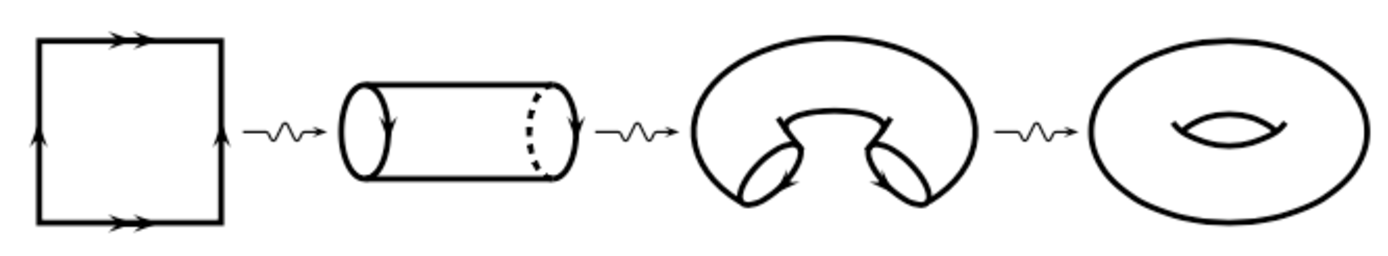
\includegraphics[width=0.8\textwidth]{figures/gluing_edges_of_square}
	\caption{Gluing the edges of a square (figure from
		\cite{tu_introduction_2011})}
	\label{fig:glue-edge-of-a-square}
\end{figure}

A quotient construction is essentially a simplifying operation. Starting from
an equivalence relation on a given set, we regard each equivalence class as a
single point. Mathematics is full of quotient constructions: quotient groups,
quotient rings, quotient spaces, and so on. If the original set is a
topological space, then in general one can always endow the quotient set with
a topology that makes the natural projection map continuous. The main result
of this section is a condition under which the quotient topological space is
still a second countable Hausdorff space.

\subsection{The Quotient Topology}

Recall that an equivalence relation on a set $S$ is reflexive, symmetric, and
transitive. The \emph{equivalence class} $[x]$ of $x\in S$ consists of all
elements of the set equivalent to $x$. An equivalence relation on a set $S$
partitions $S$ into disjoint equivalence classes. We denote the set of
equivalence classes by $S/\sim$ and call it the \emph{quotient} of $S$ under
the equivalence relation $\sim$. The \emph{natural projection map} $\pi: S\to
	S/\sim$ sends $x\in S$ to the equivalence class $[x]$.

Now suppose $S$ is a topological space. We define a topology on $S/\sim$ by
declaring $U\subset S/\sim$ to be \emph{open} if and only if its preimage
$\pi^{-1}(U)$ under the natural projection is open in $S$. Clearly,
$\emptyset$ and the quotient set $S/\sim$ itself are both open. Furthermore,
since
\begin{displaymath}
	\pi^{-1}\left(\bigcup_\alpha U_\alpha\right) = \bigcup_{\alpha}\pi^{-1}(U_\alpha)
\end{displaymath}
and
\begin{displaymath}
	\pi^{-1}\left(\bigcap_i U_i\right) =\bigcap_i \pi^{-1}(U_i),
\end{displaymath}
the collection of all open sets in $S/\sim$ is closed under arbitrary unions
and finite intersections, and hence is a topology. This is called the
\emph{quotient topology} on $S/\sim$. With this topology, $S/\sim$ is called
the \emph{quotient space} of $S$ under the equivalence relation $\sim$. Under
the quotient topology, the projection map $\pi:S\to S/\sim$ is automatically
continuous, since the preimage of an open set is open in $S$ by the very
definition of the quotient topology.


\subsection{Continuity of a Map on a Quotient}

Let $\sim$ be an equivalence relation on a topological space $S$, and let
$S/\sim$ have the quotient topology under this equivalence relation. Suppose a
function $f:S\to Y$ from the topological space $S$ to $Y$ is constant on each
equivalence class. Then it induces a map $\bar{f}: S/\sim \to Y$ given by
\begin{displaymath}
	\bar{f}([p]) = f(p)\quad \text{for $p\in S$}.
\end{displaymath}
In other words, there is a \emph{commutative diagram}
\begin{displaymath}
	\begin{tikzcd}
		S \arrow[r,"f"]\arrow[d,"\pi"] & Y.\\
		S/\sim \arrow[ru,"\bar{f}"]
	\end{tikzcd}
\end{displaymath}

\begin{proposition}
  \label{prop:continuous-of-quotient-map}
	The induced map $\bar{f}: S/\sim\to Y$ is continuous if and only if the
	map $f: S\to Y$ is continuous.
\end{proposition}

\begin{proof}
	\begin{itemize}
		\item [($\Longrightarrow$)] If $\bar{f}$ is continuous, then the
		      composite $\bar{f}\circ \pi$ is continuous, so $f$ is continuous as
		      well.
		\item [($\Longleftarrow$)] Suppose $f$ is continuous. Let $V$ be an
		      open set in $Y$; then $f^{-1}(V)=\pi^{-1}(\bar{f}^{-1}(V))$ is an
		      open set in $S$. By the definition of the quotient topology,
		      $\bar{f}^{-1}(V)$ is open in $S/\sim$. Since $V$ was arbitrary,
		      $\bar{f}: S/\sim\to Y$ is a continuous map.
	\end{itemize}
\end{proof}

This proposition gives a useful criterion for checking whether a map
$\bar{f}$ on the quotient space $S/\sim$ is continuous: simply lift $\bar{f}$
to $f := \bar{f}\circ \pi$ and check whether the lifted map $f$ is continuous
on $S$.


\subsection{Identification of a Subset to a Point}
If $A$ is a subspace of $S$, we define a relation $\sim$ on $S$ by
\begin{displaymath}
	x\sim x \quad \text{for $x\in S$}
\end{displaymath}
and
\begin{displaymath}
	x\sim y \quad \text{for $x,y\in A$}
\end{displaymath}
This is an equivalence relation on $S$. We say that the quotient space
$S/\sim$ is obtained from $S$ by \emph{identifying $A$ to a point}.

\begin{example}
	Let $I$ be the unit interval $[0,1]$, and let $I/\sim$ be the quotient
	space obtained from $I$ by identifying the two points $\{0,1\}$ to a
	single point. Denote the unit circle in the complex plane by $S^1$. Then
	the function $f:I\to S^1$, $f(x)=\exp(2\pi i x)$, takes the same value
	at $0$ and $1$, and hence induces a map $\bar{f}: I/\sim \to S^1$ (see
	Figure \ref{fig:circle-as-quotient-of-interval})

	\begin{figure}[ht]
		\centering
		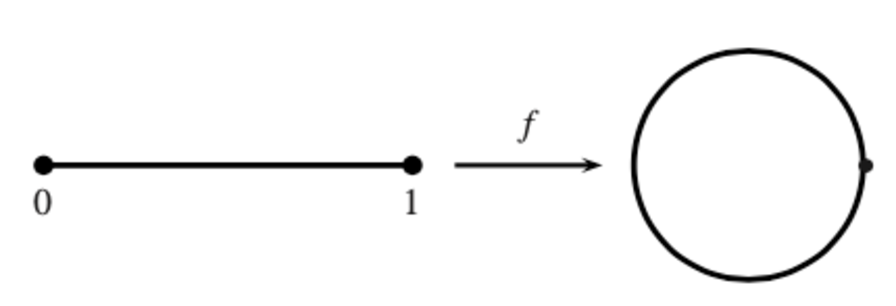
\includegraphics[width=0.6\textwidth]{figures/circle_as_quotient_of_interval}
		\caption{The unit circle as a quotient of the unit interval (figure
			from \cite{tu_introduction_2011})}
		\label{fig:circle-as-quotient-of-interval}
	\end{figure}
\end{example}


\begin{proposition}
  \label{prop:interval-to-s1}
	The map $\bar{f}:I/\sim \to S^1$ is a homeomorphism.
\end{proposition}

\begin{proof}
	Since $f$ is continuous, $\bar{f}$ is also continuous by Proposition
	\ref{prop:continuous-of-quotient-map}. Clearly $\bar{f}$ is a bijection.
	As the image of the compact set $I$ under a continuous map, the quotient
	$I/\sim$ is compact. Hence $\bar{f}$ is a continuous bijection from the
	compact space $I/\sim$ to the Hausdorff space $S^1$, so by Corollary
	\ref{cor:from-compact-to-hausdorff}, $\bar{f}$ is a homeomorphism.
\end{proof}


\subsection{A Necessary Condition for a Hausdorff Quotient}

In general, a quotient construction need not preserve the Hausdorff property
or second countability. In fact, since every one-point set in a Hausdorff
space is closed, if $\pi: S\to S/\sim$ is a projection and the quotient space
$S/\sim$ is Hausdorff, then for every $p\in S$, its image $\{\pi(p)\}$, as a
one-point set in $S/\sim$, should be closed in $S/\sim$. By the continuity of
$\pi$, the preimage $\pi^{-1}(\{\pi(p)\})=[p]$ should be a closed set in $S$.
This gives a necessary condition for a quotient space to be Hausdorff.

\begin{example}
	Define an equivalence relation on $\RR$ by regarding the open interval
	$(0,\infty)$ as a single point. Then the quotient space $R/\sim$ is not
	Hausdorff, because the equivalence class $(0,\infty)$ under $\sim$ is
	not a closed set in $\RR$.
\end{example}


\subsection{Open Equivalence Relations}

In this section we follow the approach of Boothby to derive conditions for a
quotient space to be Hausdorff or second countable. Recall that a map $f:X\to
	Y$ between topological spaces is \emph{open} if the image under $f$ of
every open set is open.

\begin{definition}
	An equivalence relation $\sim$ on a topological space $S$ is called
	\emph{open} if the projection map $\pi: S\to S/\sim$ is an open map.
\end{definition}

In other words, an equivalence relation on $S$ is open if and only if for
every open set $U\subset S$, the set
\begin{displaymath}
	\pi^{-1}(\pi(U)) = \bigcup_{x\in U}[x]
\end{displaymath}
is open.

\begin{figure}[ht]
	\centering
	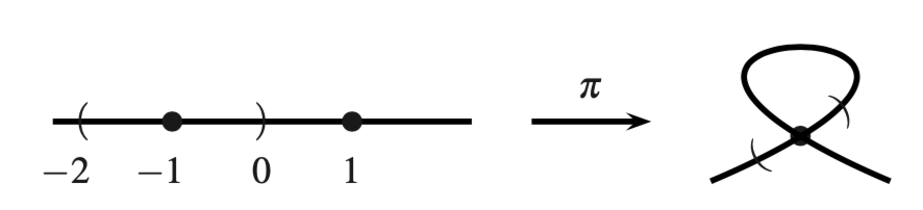
\includegraphics[width=0.6\textwidth]{figures/projection_not_open}
	\caption{A projection map that is not open (figure from
		\cite{tu_introduction_2011})}
	\label{fig:projective-is-not-open}
\end{figure}

\begin{example}

	The projection map onto a quotient space is in general not open. For
	example, let $\sim$ be the equivalence relation on $\RR$ that identifies
	$1$ and $-1$, and let $\pi:\RR\to\RR/\sim$ be the projection map (see
	Figure \ref{fig:projective-is-not-open}).

	The map $\pi$ is open if and only if for every open set
	$V\subset\RR$, its image $\pi(V)$ is open in $\RR/\sim$; by the
	definition of the quotient topology this requires that
	$\pi^{-1}(\pi(V))$ be open in $\RR$. Now take $V=(-2,0)\subset\RR$; then
	\begin{displaymath}
		\pi^{-1}(\pi(V)) = (-2,0)\cup \{1\},
	\end{displaymath}
	which is not an open set in $\RR$. Hence the projection map
	$\pi:\RR\to\RR/\sim$ is not an open map.

\end{example}

Given an equivalence relation $\sim$ on $S$, let $R$ be the subset of $S\times
	S$ defined by
\begin{displaymath}
	R=\{(x,y)\in S\times S\, |\, x\sim y\}.
\end{displaymath}
We call $R$ the \emph{graph} of the equivalence relation $\sim$.


\begin{figure}[ht]
	\centering
	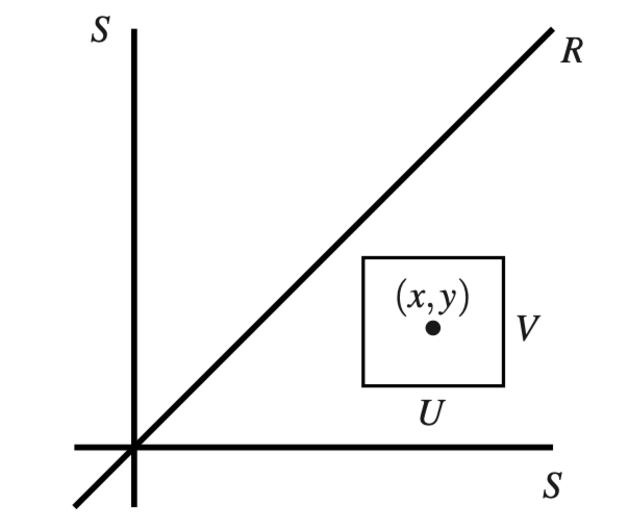
\includegraphics[width=0.4\textwidth]{figures/graph_of_equivalence_relation}
	\caption{The graph $R$ of an equivalence relation and an open set
		$U\times V$ disjoint from $R$ (figure from
		\cite{tu_introduction_2011})}
	\label{fig:graph-of-equivalence-relation}
\end{figure}

\begin{theorem}
  \label{thm:quotient-be-hausdorff}

	Let $\sim$ be an open equivalence relation on a topological space $S$.
	Then the quotient space $S/\sim$ is Hausdorff if and only if the graph
	of the equivalence relation $\sim$ is closed in $S\times S$.

\end{theorem}

\begin{proof}
	We have the following chain of equivalent statements:

	$R$ is closed in $S\times S$

	$\Longleftrightarrow$ $S\times S- R$ is open in $S\times S$

	$\Longleftrightarrow$ for every $(x,y)\in S\times S-R$, there exists a
	basic open set $U\times V$ containing $(x,y)$ such that $(U\times V)\cap
		R = \emptyset$ (see Figure \ref{fig:graph-of-equivalence-relation})

	$\Longleftrightarrow$ for every pair $x\not\sim y$ in $S$, there exist a
	neighborhood $U$ of $x$ and a neighborhood $V$ of $y$ such that no
	element of $U$ is equivalent to any element of $V$

	$\Longleftrightarrow$ for any two points $[x]\neq [y]$ in $S/\sim$,
	there exist a neighborhood $U$ of $x$ and a neighborhood $V$ of $y$ such
	that $\pi(U)\cap \pi(V)=\emptyset$ (in $S/\sim$). \qquad\qquad (*)

	We now show that the last statement (*) is equivalent to $S/\sim$ being
	Hausdorff. First suppose (*) holds. Since $\sim$ is an open equivalence
	relation, $\pi(U)$ and $\pi(V)$ are disjoint open sets in $S/\sim$
	containing $[x]$ and $[y]$ respectively. Hence $S/\sim$ is a Hausdorff
	space.

	Conversely, suppose $S/\sim$ is Hausdorff. Let $[x]\neq [y] \in
		S/\sim$. Then there exist two disjoint open sets $A$ and $B$ in
	$S/\sim$ such that $[x]\in A$, $[y]\in B$. Since the projection map is
	surjective, we have $A=\pi(\pi^{-1} A)$ and $B=\pi(\pi^{-1}B)$. Set
	$U=\pi^{-1}A$ and $V = \pi^{-1}B$. Then $x\in U$, $y\in V$, and
	$A=\pi(U)$, $B=\pi(V)$ are disjoint open sets in $S/\sim$.
\end{proof}

If the equivalence relation $\sim$ is equality, then the quotient space
$S/\sim$ is $S$ itself and the graph $R$ is the diagonal
\begin{displaymath}
	\Delta = \{(x,x)\in S\times S\}.
\end{displaymath}
In this case, Theorem \ref{thm:quotient-be-hausdorff} becomes the following
well-known characterization of Hausdorff spaces in terms of their diagonals.

\begin{corollary}\label{cor:quotient-space-diagonal}
	A topological space $S$ is Hausdorff if and only if its diagonal
	$\Delta\in S\times S$ is closed.
\end{corollary}

\begin{theorem}
	Let $\sim$ be an open equivalence relation on a topological space $S$,
	with projection map $\pi : S\to S/\sim$. If $\mathcal{B} = \{B_\alpha\}$
	is a basis for $S$, then its image $\{\pi(B_\alpha)\}$ is a basis for
	$S/\sim$.
\end{theorem}

\begin{proof}
	Since $\pi$ is an open map, $\{\pi(B_\alpha)\}$ is a collection of open
	sets in $S/\sim$. Let $W$ be an open set in $S/\sim$ with $[x]\in W$,
	$x\in S$. Then $x\in\pi^{-1}(W)$. Since $\pi^{-1}(W)$ is open, there
	exists a basic open set $B\in\mathcal{B}$ such that
	\begin{displaymath}
		x\in B\subset \pi^{-1}(W).
	\end{displaymath}
	Then
	\begin{displaymath}
		[x]=\pi(x)\in\pi(B)\subset W,
	\end{displaymath}
	which proves that $\{\pi(B_\alpha)\}$ is a basis for $S/\sim$.
\end{proof}

\begin{corollary}\label{cor:quotient-second-countable}
	If $\sim$ is an open equivalence relation on a second countable space
	$S$, then the quotient space $S/\sim$ is second countable.
\end{corollary}

\newpage
